\chapter{Future}
A lot of big software projects (such as the Level-1 Configuration Editor and
the Level-1 page) rely on the TS.
Some of these projects are starting to benefit from the changes made to the TS,
and some of them are scheduled for a complete overhaul using the TS redesign as
a template.

Some things did not make it into the TS, because of backward-compatibility problems
or time issues.
However, as time goes on, the need to keep compatibility with legacy systems will
fade away. And some improvements may yet become possible.

\section{Dojo-free TS release}
At some point, all legacy (Dojo) panels will have been migrated to Polymer.
When this has occurred, legacy code can be removed from the TS.

A lot of code can be removed. The Dojo component classes, legacy session logic,
the legacy event system, etc.

Furthermore, Dojo can be removed from the front-end interface. This is expected
to bring a noticeable speed improvement to the initial page load.

At this point, the TS can also be prepared to take on a next framework, where this
time Polymer will be considered legacy code.

\section{HTML5 WebSocket}
A WebSocket is a full-duplex HTTP-like connection between a web browser and a web server.
Both the client and the server must support this protocol before such a connection
can be set up.

This allows for very efficient communication between client and server, and will
be especially useful when the server has frequently changing data to serve to the
client.
Traditionally this has been achieved using various sort of polling, which puts
unnecessary load on the server and the network.

This connection will also allow the web browser to receive updates near-instantaneous.

Currently, the most CPU intensive tasks in the TS interface belong to the auto-update
logic. This would be drastically reduced when implementing WebSockets.

\section{PRPL}
The PRPL\cite{PRPL} pattern is a software pattern for web apps designed by Google and stands for:
\begin{itemize}[noitemsep]
\item \textbf{Push} critical components for initial page load
\item \textbf{Render} the initial page
\item \textbf{Pre-cache} other components of the interface
\item \textbf{Lazy-load} needed components
\end{itemize}

It uses Web Components, HTML Imports, Service Workers, and HTTP/2 to accomplish
all these. The TS already uses two of them, Web Components and HTML Imports.
The two others that didn't make it into the TS are explained here in a bit more
detail.

\subsection{HTTP/2 Server Push}
Using HTTP/2, the server can interpret requested resources and decide to not only
return the requested resource to the client, but also provide the user with
additional resources related to the requested resource.

This is useful on the first page load, where a web browser requests the initial
page (usually `index.html`). This file very often contains references to other
resources such as CSS or JavaScript files.
Normally the web browser needs to make another request for each of these
resources.
HTTP/2 can multiplex these related resources along with the originally requested
resource over the same connection.
This severely reduces network latencies, as everything is returned
in one payload.
This effect is demonstrated in image \ref{fig:http1_server} and \ref{fig:http2_server}.

\begin{figure}
  \centering
  \begin{minipage}[t]{0.49\textwidth}
    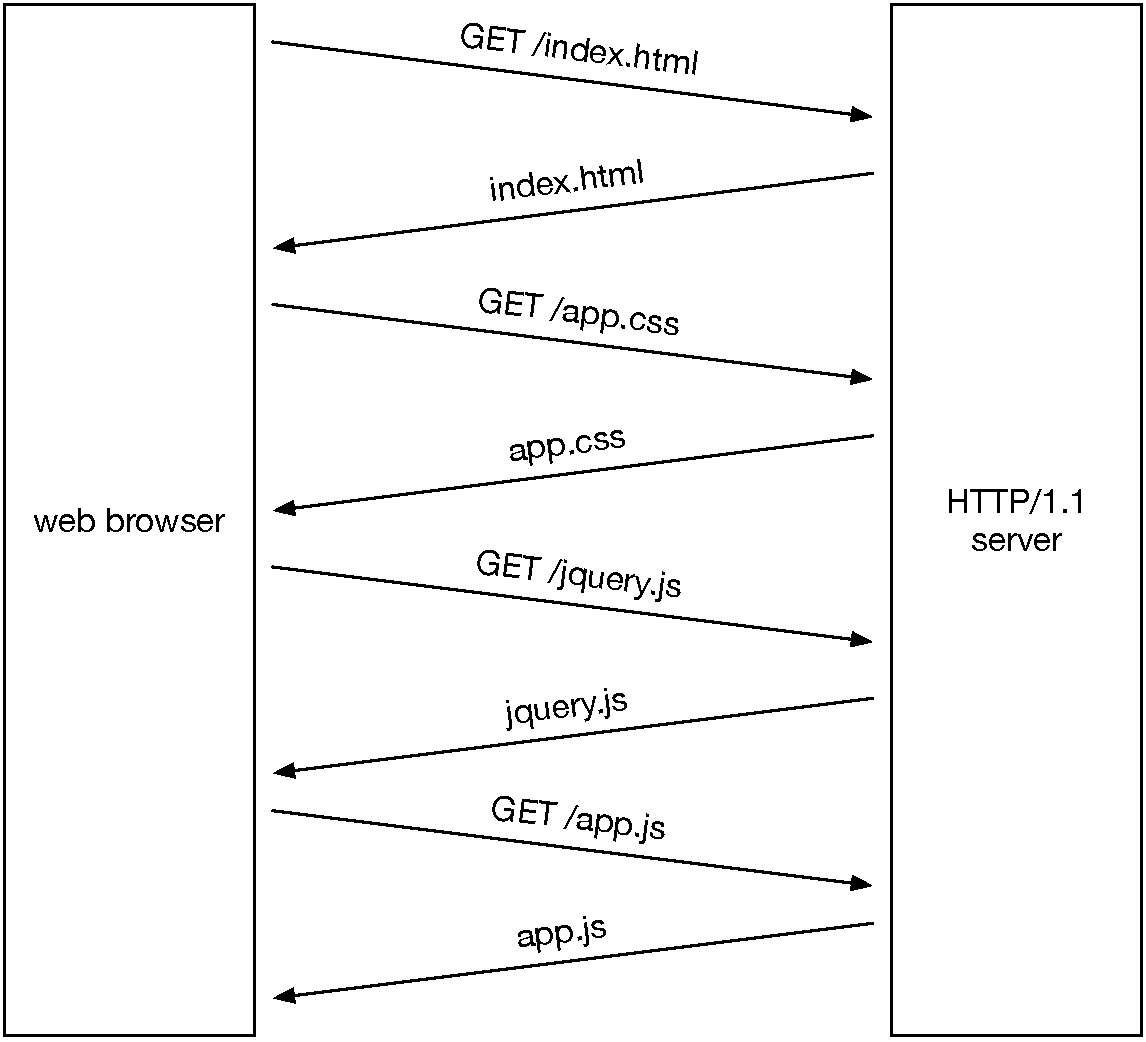
\includegraphics[width=\textwidth]{images/http1_server}
    \caption{A common request/response diagram when using a HTTP/1.1 server}
    \label{fig:http1_server}
  \end{minipage}
  \hfill
  \begin{minipage}[t]{0.49\textwidth}
    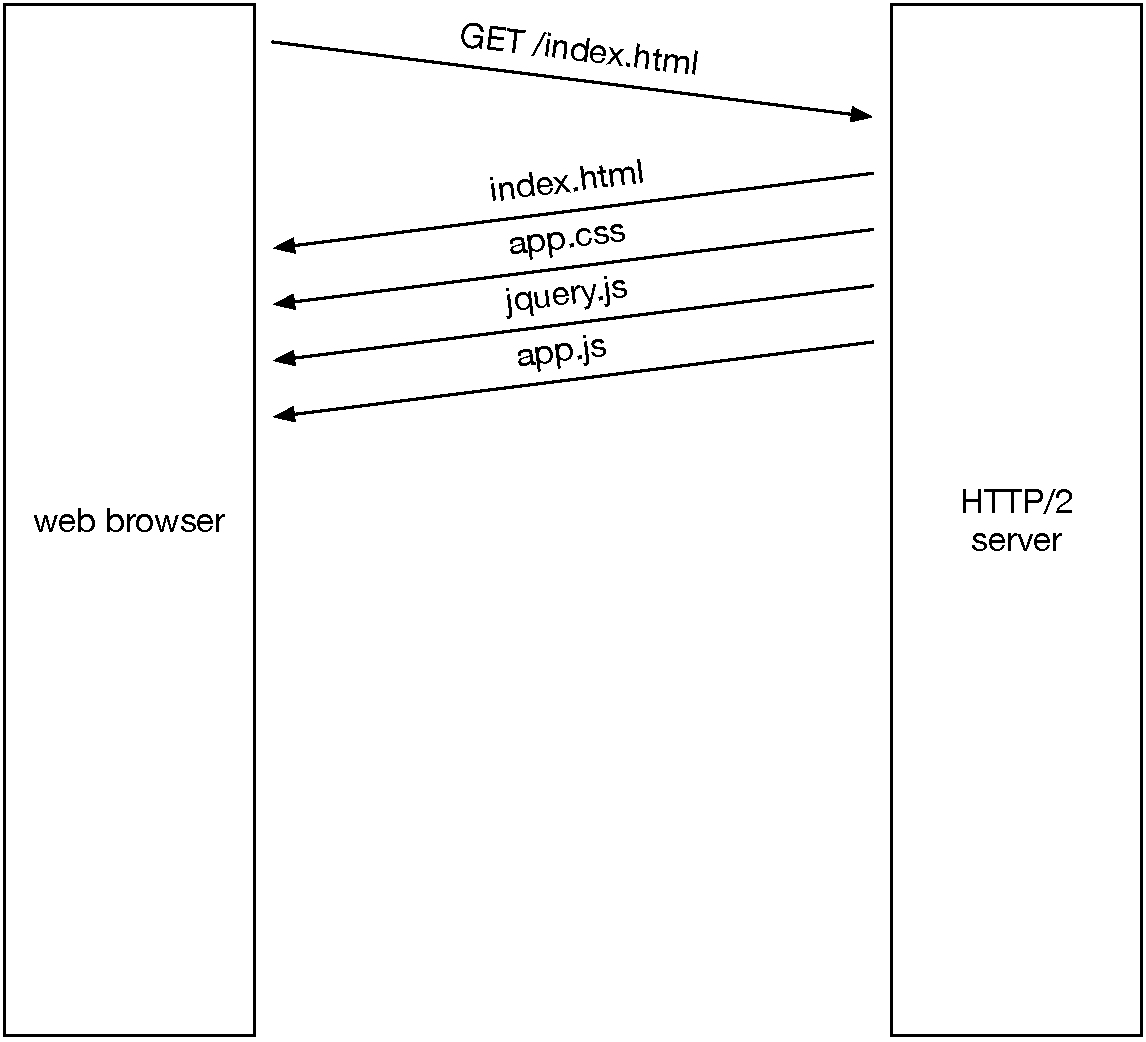
\includegraphics[width=\textwidth]{images/http2_server}
    \caption{A common request/response diagram when using a HTTP/2 server with Server Push}
    \label{fig:http2_server}
  \end{minipage}
\end{figure}

\subsection{HTML5 Service Worker}
A Service Worker is a JavaScript file that is run in the browser as a separate
thread.
Unlike traditional JavaScript files, this file has no access to the DOM or any
global variables like `document` or `window`. This file runs on a different scope.

A Service Worker runs in between the browser and the network. It is able to
intercept requests and modify them. It can even provide a response, thereby
completely bypassing the server and the network.

It also has full control over the browser cache. So the interface can programmatically
control what is put in the cache and when it is served or renewed.
This is shown visually in image \ref{fig:service_worker}.

\begin{figure}
  \centering
  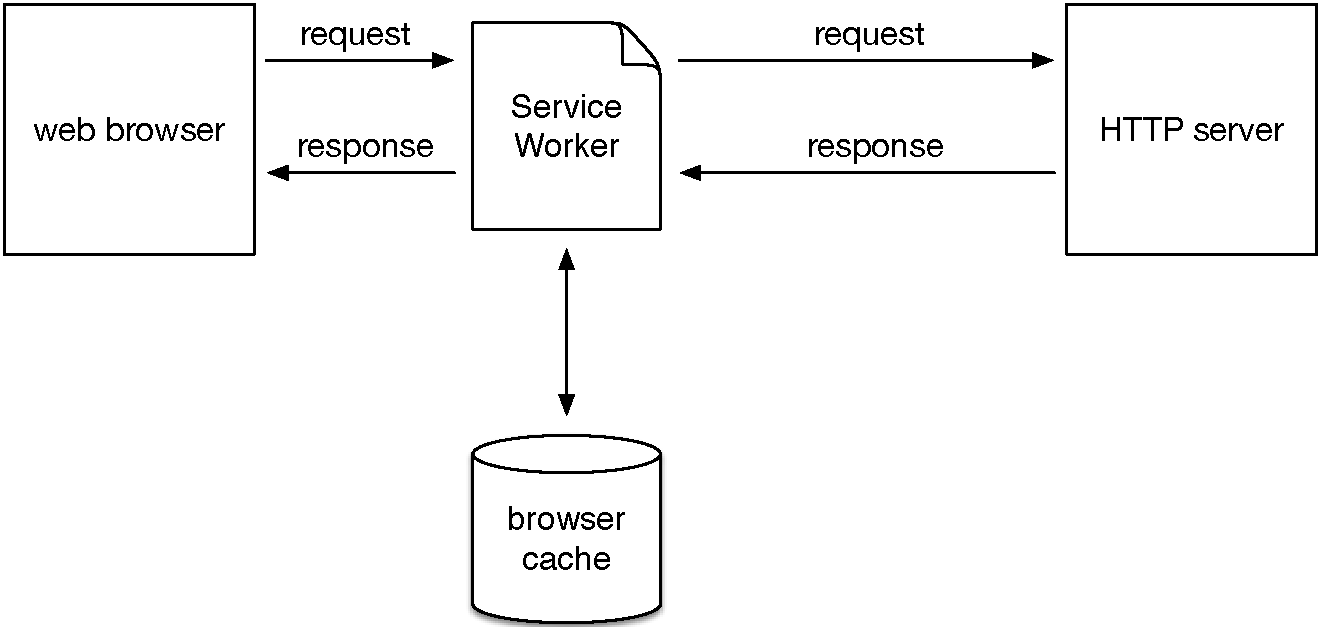
\includegraphics[width=\textwidth]{images/service_worker}
  \caption{Logical location of the Service Worker in a web browser}
  \label{fig:service_worker}
\end{figure}

This enables the interface to do two thing that were previously impossible, but
very useful.

The first is pre-caching. When the initial page load is done, the Service Worker
can silently pull resources from the web server before they are actually needed.
This will make interacting with the application a lot faster.

The second thing is offline functionality, and is a more elaborate version of
pre-caching.
When enough resources are pulled into the cache, the interface does not need the
web server anymore: in some cases (including the initial page load), the interface can work without an internet connection.

This will completely remove the need for network requests (except for receiving
new data): static resources (and data) are kept client-side and do not put a
load on the network anymore, vastly increasing performance.
